\documentclass{llncs2e/llncs}

% \usepackage{makeidx}  % allows for indexgeneration
\usepackage{verbatim}
\usepackage[utf8]{inputenc}
\usepackage{graphicx}
\usepackage{bibentry}
\usepackage[numbers]{natbib}

\title{An Argumentative Approach for a BDI Agent} % tentativo
        
\author{I\~{n}aki Garay \and      % igarai@gmail.com
        Diego Marcovecchio \and   % diegomarcov@gmail.com
        Leonardo Molas \and       % leos.molas@gmail.com
        Emiliano Montenegro \and  % emm.montenegro@gmail.com
        Fernando Sisul \and       % fsisul@gmail.com
        Manuel Torres \and        % jmtorresluc@gmail.com
        Sebastián Gottifredi \and % sebastian.gottifredi@gmail.com
        Alejandro García \and     % ajg@cs.uns.edu.ar
        Diego Martínez \and       % dcm@cs.uns.edu.ar
        Guillermo Simari          % grs@cs.uns.edu.ar
        }

\institute{Universidad Nacional del Sur \email{\{igarai,diegomarcov,leos.molas,emm.montenegro,fsisul,jmtorresluc\}@gmail.com,\\\{sg,ajg,dcm,grs\}@cs.uns.edu.ar}}

\begin{document}

\maketitle

\begin{comment}
\pagestyle{headings}  % switches on printing of running heads
\addtocmark{Hamiltonian Mechanics} % additional mark in the TOC
figuras
- la arquitectura del agente
- la arquitectura del programa
- ejemplo del fog of war y coloreo
meter una buena explicacion de la arquitectura bdi en la parte de diseño

- arquitectura
- argumentacion
- estrategias
- percept server
\end{comment}

\begin{abstract}
    This report presents the design and results of the d3lp0r multi-agent system 
    developed by the LIDIA team for the 2011 Multi-Agent Programming Contest.
    The d3lp0r agents use a BDI architecture extended with planning and 
    argumentation (via Defeasible Logic Programming) to model a cooperating team 
    operating in a dynamic and competitive environment.

    In particular, the main goal of this report is to describe the chosen 
    architecture, the communication scheme and the way argumentation was put to 
    use in the agent's reasoning process and the technical details thereof.
\end{abstract}

\section{Introduction}

    The LIDIA (Laboratorio de Investigación y Desarrollo en Inteligencia 
    Artificial, Artificial Intelligence Research and Development Laboratory) 
    research group was established in 1992 at the Universidad Nacional del Sur. 
    The d3lp0r team was formed incorporating six graduate students, two Ph.D. 
    students and three professors. The undergraduate students fully developed the 
    system, while the Ph.D. students and professors provided guidance. The group's 
    main motivation was to apply argumentation via defeasible logic programming 
    (DeLP) in a BDI based agent, in the context of a multi-agent gaming situation, 
    and to test the integration of the different technologies used.

    Experience from a previous instance of the MAPC was shared with our teams by 
    members of the ARGONAUTS team from Universität Dortmund. Although the initial 
    plan was to run tests against other agent teams prior to the competition, time 
    constraints acted against this.

\begin{comment}
PREGUNTAS {
1. What was the motivation to participate in the contest?
2. What is the history of the team?
3. What is the name of your team?
4. How many developers and designers did you have?  At what level of education 
are your team members?
5. From which field of research do you come form?  Which work is related?
}
\end{comment}

\section{Preliminaries}

    The \texttt{d3lp0r} system was developed in the context of the 2011 edition 
    of the Multi-Agent Programming Contest hosted by the University of 
    Clausthal. 

    The simulation scenario is represented as an undirected graph, in which 
    nodes are valid agent locations weighted by value, and edges are valid
    transitions weighted by cost. 
    Agent state includes energy, health, and strength parameters. Agent percepts
    include visible nodes, edges, and other agents. 
    Each agent is assigned a role in the simulation (Explorer, Saboteur,
    Repairer, Sentinel and Inspector) which determines its valid actions and
    initial maximum values for the agent state parameters. 
    Actions in general have an energy cost, movement action costs depend on edge
    weights, successful attack actions decrease enemy agent's health subject to
    a comparison of their strength attributes. Certain actions may cause further
    information to be included in subsequent percepts. 

    A match consists of several simulations, and each simulation proceeds as
    a series of steps. In each step, each agent is provided with a percept with
    partial information about the current simulation state and is
    queried for its action. 

    The goal is to maximize the score function each step. A team is awarded
    points according to the value of the nodes controlled by the team, and
    in addition certain achievements. Agents may control more nodes than 
    those they are positioned in by forming zones, groups of nodes under the
    influence of a team determined by a graph coloring algorithm specified in
    the scenario description. 

    The final score for a team is the sum of points over all steps; at the end
    of the match, the team with the most points is the winner.

\section{System Analysis and Design}

\begin{comment}
PREGUNTAS {
1. If some multi-agent system methodology such as Prometheus, O-MaSE, or 
Tropos was used, how did you use it? 
   If you did not what were the reasons?
2. Is the solution based on the centralisation of coordination/information on 
a specific agent?
   Conversely if you plan a decentralised solution, which strategy do you plan 
to use?
3. What is the communication strategy and how complex is it?
4. How are the following agent features considered/implemented: autonomy, 
proactiveness, reactiveness?
5. Is the team a truly multi-agent system or rather a centralised system in 
disguise?
6. How much time (man hours) have you invested (approximately) for 
implementing your team?
7. Did you discuss the design and strategies of your agent team with other 
developers? 
   To which extent did your test your agents playing with other teams?
}
\end{comment}

    Despite many man-hours dedicated to design in the early stages of
    the competition, the development team's lack of experience in multi-agent
    systems made necessary several changes and additions. 
    Despite this, our approach was more than satisfying, resulting to be
    modular, correct and in close correspondence with the literature.

\subsection{Agent Design}

    The solution follows a decentralised architecture in which agents run 
    completely decoupled in different processes while sharing nothing. Percepts 
    are communicated among agent members of the team via a broadcast mechanism 
    developed as part of the multi-agent system. This design was chosen for its 
    minimal complexity.

    Agents are completely autonomous meaning that decision-making takes place 
    individually at the agent level, with no intervention from human operators or 
    a central intelligence agency within the system, and that decisions made by an 
    agent are influenced solely by the current simulation state and the results of 
    previous steps.
    The agent architecture developed is based on the BDI model \cite{Rao:1991}, 
    and is explained in detail in further sections.

    No design methodology specific to multi-agent systems was used. However, 
    the implementation was conducted using a simplified XP (extreme programming) 
    methodology.


\section{Software Architecture}

\begin{comment}
PREGUNTAS {
1. Which programming language did you use to implement the multi-agent system?
2. Did you use multi-agent programming languages? Why or why not to use a 
multi-agent programming language?

3. How have you mapped the designed architecture (both multi-agent and 
individual agent architectures) to programming codes i.e., how did you 
implement specific agent-oriented concepts and designed artifacts using the 
programming language?
4. Which development platforms and tools are used? How much time did you 
invest in learning those?
5. Which runtime platforms and tools (e.g. Jade, AgentScape, simply Java, 
....) are used? How much time did you invest in learning those?
6. What features were missing in your language choice that would have 
facilitated your development task?
7. What features of your programming language has simplified your development 
task?
8. Which algorithms are used/implemented?
9. How did you distribute the agents on several machines? And if you did not 
please justify why.
10. To which extend is the reasoning of your agents synchronized with the 
receive-percepts/send-action cycle?
11. What part of the development was most difficult/complex? What kind of 
problems have you found and how are they solved?
12. How many lines of code did you write for your software?
}
\end{comment}

\begin{figure}
%\centering
%  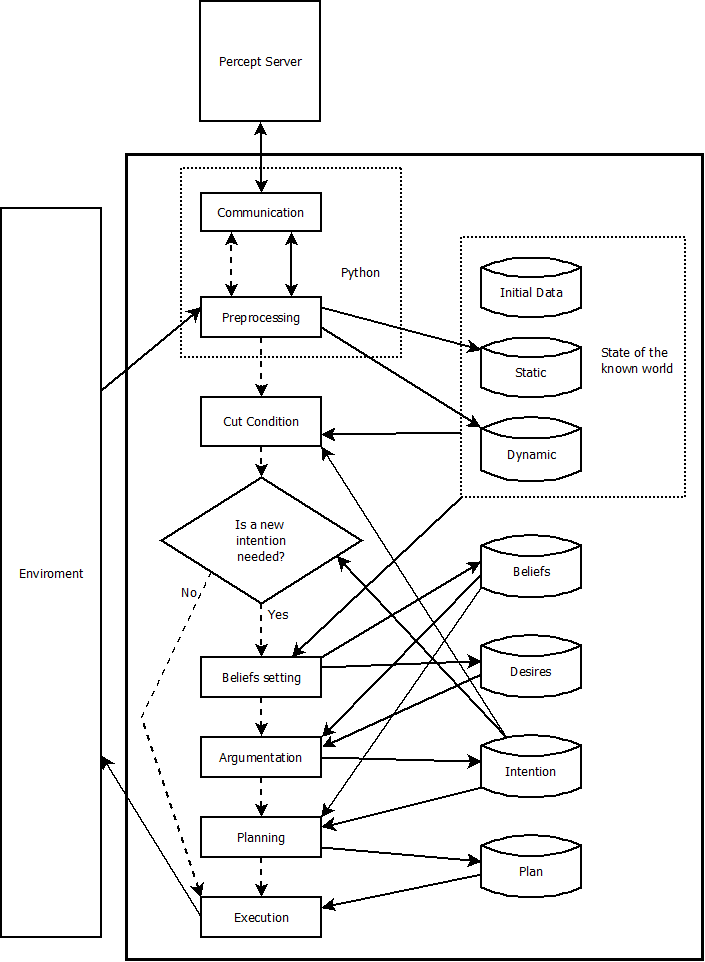
\includegraphics[width=\textwidth]{agent_architecture2.png}
%    \caption{Agent architecture in a flow chart-like diagram. 
%    Dashed arrows represent process flow, solid lines represent data flow.}
%\label{fig:architecture}
\end{figure}

    In Fig. \ref{fig:architecture}, we sketch the architecture of our agent, 
    i.e. its interactions with the servers (MASSIM, and our Percept Server), 
    and its internal components.
 

\subsection{Architecture implementation}



%Aca va toda la bola de explicacion del dibujito

    The first part of the architecture is the Python part, that handles all the 
    communication with the servers. It first opens a TCP/IP connection with the 
    MASSIM server, and authenticates. Then it does the same with our Percept 
    Server, that has to be running. It waits for all the agents, and then 
    everything is set to start the simulation.

\subsubsection{Percept-act loop.}

    When the first action-request message is received, this loop starts. It 
    first processes the perception, and then sends it to the Percept Server. 
    This waits for all the other agents' perceptions, merges them, and then sends 
    back a new version that cointains everything that has been seen by the agent 
    teammates, but not by itself. Finally, this global perception is asserted 
    into Prolog. 
    As it will be explained below, this part of the program constitutes the 
    decision making module. Therefore, the Python part will query it, for the
    next action to be performed by the agent.
    
\subsubsection{Action requested.}

    As seen in the Figure \ref{fig:architecture}, after the Python part, comes 
    all the processing in Prolog. The perception is already in the knowledge 
    base, that is formed by the ``static'' and ``dynamic'' data. 

    If the agent already has an intention stored, the \textit{cut condition}
    checks whether it makes sense to keep trying to fulfill it. It is a series
    of simple conditions that review the state of the world.

    Then, if there is not any commited intention, or the cut condition decides 
    it is not interesting to keep it, the \textit{beliefs setting process} is 
    started. It generates the possible desires for this step, according to what 
    is stored in the knowledge base, and, for each one of them, the beliefs 
    needed. 
    The decision-making module is implemented in DeLP, a defeasible logic 
    programming language that uses argumentation to reason with conflicting
    information. 
    Given the set of possible 
    desires and beliefs set by the previous module, it selects the best desire, 
    returning it as the intention that the agent commits to achieve.

    All the plans for all the desires were previously calculated and stored as 
    beliefs, since the amount of steps that they take is used by the 
    argumentation module. The \textit{planning} module selects the one 
    corresponding to the selected intention, and stores it. Then, the 
    execution module only gets the plan, and returns to Python the first 
    action in it.

    However, if the process flow comes from the other branch of Fig. \ref{
    fig:architecture} (that is, after the cut condition, the agent has an 
    intention), the execution is not that simple. Since skipping the decision-
    taking makes this branch insignificant in terms of time, we decided to 
    recalculate the plan. This might help us when a better path is discovered, 
    even though this is unlikely.

    Back again in Python, with the returned action, an XML is formed to be sent 
    to the server.

\subsection{Programming languages, platforms and tools}

    The agent system was implemented using Python 2.7 and SWI Prolog 5.10.5. DeLP 
    \cite{Garcia:2004a}, a defeasible logic programming language, was used as a 
    service within Prolog. 
    Language integration was achieved using the \textit{pyswip}\ library, 
    calling Prolog predicates from Python. The implementation of Defeasible 
    Logic Programming (DeLP) by the LIDIA was used for the deliberative 
    process. They were well-known at the start of the project, and were chosen 
    for precisely those reasons.
    
    No multi-agent programming languages/platforms/frameworks were used due to 
    previous experience indicating a general lack of flexibility, and a lack of 
    familiarity on behalf of the development team.
    
    Both Linux and the Windows operating system were used as development 
    platforms, since the language runtimes chosen for implementation were 
    portable. Some caveats were encountered however.

    We used \textit{git}\ as our revision control system. In general, we did 
    not spend much time in learning it, since some of us had already worked 
    with it.
    
\subsubsection{DeLP.}
    
    \newcommand{\drule}[2]{\mbox{$ #1\; \defleftarrow \; #2$}}
    \newcommand{\defleftarrow}{{\raise1.5pt\hbox{\tiny\defleft}}}
    \newcommand{\defleft}{\mbox{---\hspace{-1.5pt}\raise.05pt\hbox{$<$}}}

    In DeLP\cite{Garcia:2004a}, knowledge is represented using facts, strict rules
    and defeasible rules. Facts and strict rules are ground literals representing
    firm information that can not be challenged. \textit{Defeasible Rules}
    (d-rules) are denoted $\drule{L_0}{L_1, \ldots, L_n}$ (where $L_i$ are literals)
    and represent tentative information. These rules may be used if nothing could
    be posed against it. A d-rule \textit{``\drule{Head}{Body}''} expresses that
    \textit{``reasons to believe in Body give reasons to believe in Head''}. A DeLP
    program is a set of facts, strict rules and defeasible rules. 

    {\it Strong negation} is allowed in the head of program rules, and hence, may
    be used to represent contradictory knowledge. From such a program contradictory
    literals could be derived, however,  the set of facts and strict rules must
    possess certain internal coherence (it has to be non-contradictory). 

    To deal with contradictory information, in DeLP, \emph{arguments} for
    conflicting pieces of information are built and then compared to decide which
    one prevails. The prevailing argument is a \emph{warrant} for the information
    that it supports.

    In DeLP, a query $L$ is \emph{warranted} from a program if a \emph{non-defeated}
    argument that supports $L$ exists. %\Arg\ 



\subsubsection{Benefits.}
    
    Python's amenity to rapid application development and 'batteries-included 
    philosophy' facilitated implementing the communication layer to the MASSim 
    server, parsing of peceptions, rapid addition of planned features and bug 
    correction.

    We made use of Prolog's declarative nature to model states of the world, and it 
    also made more straightforward to implement search algorithms like Uniform Cost 
    Search, and Depth First Search. The zone-coloring algorithm was also 
    implemented in Prolog.
    
    DeLP's capability to deal with conflicting pieces of information was also very
    helpful in order to implement the decision-making module.
    
    Initial plans were to distribute agents on several machines. Each agent runs 
    as a separate process, and communicates with others via TCP sockets. After 
    some experience and benchmarking, agents were run on one machine, due to 
    performance issues. 
    Having the choice was a benefit of the proposed design.

\subsubsection{Problems encountered.}

    The most difficult problems were related to optimization. Much of our time was 
    spent in reducing the complexity of our algorithms, and the times they 
    were called.

    For the coloring algorithm, we added several improvements, for both 
    optimization and correctness. In essence, since we only had an incomplete 
    version of the full map in every step, we added the concept of ``fog of war`'' 
    to the agents, assuming always in a pessimistic way. 

    For both search algorithms, the Depth First Search and the Uniform Cost 
    Search, we added conditions that could cut several branches, when they were 
    expanding to unwanted nodes. This conditions were set by the caller, since 
    they depend on the context of the problem.

    For the UCS, we first used a simple stack implemented with a list, to keep 
    track of the frontier, because of Prolog's inability to work with arrays. This 
    would have allowed us to develop a heap data structure, to be used in a 
    priority queue. Lately, we found a Prolog library that implemented this data 
    structure, and the migration was pleasantly straightforward.

    Finally, for this last algorithm too, we added an important optimization 
    that allowed us to call it several times, with the virtual cost of only one 
    call. It was done using memoization, and a more thoughtful invocation.

\section{Stategies, Details, and Statistics}

\subsection{Strategy}
    The main strategy of the team consists of detecting profitable zones from the 
    explored vertices, and positioning the agents correctly to maintain, defend 
    and expand the zones. 
    
    Our agents do not change their behavior during runtime. It is actually very 
    easy to add this feature, but we had not enough time to implement it.
    
    Achievements are not taken under consideration. However, agents can
    achieve a significant number of them, since this behavior is implicitly 
    implemented.
    
\subsubsection{Zone conquering.}
    
    If an agent is not being part of any zone, it tries to regroup with a partner. 
    When a zone is formed, and the agent is part of it, for each potentially 
    beneficial neighbor node, the agent calculates how much points would they win 
    if it moves, and that information is used by the decision taking module.
    Agents make no assumption about the map topology. They will prefer higher 
    valued nodes over lower ones.

    If the expansion intention explained is selected and carried on, then a new 
    better zone is implicitly conquered.

\subsubsection{Attacking and defending.}
    
    Both attacking and defense are implicitly implemented. Sabouteurs attack 
    enemies that are near, so they might attack them if they enter our team's 
    zone, as well as when they are in their zone. Any other agent of another role
    can go to a node that has, for example, two agents, one for each team, in order
    to expand the zone, occupying the contested node, and implicitly defending it.
    
\subsection{Implementation}

    Here are the details of the implementation of the different parts of the
    agents.

\subsubsection{Path planning.}

    Path planning is implemented with an Uniform Cost Search 
    \cite{Russell:2003:AIM:773294}. 
    What we tried to minimize was the amount of steps required to achieve the 
    goal, rather than the spent energy. 
    The returned result is the list of actions to be done, rather than the list of 
    nodes.
    
    Since this algorithm can be called several times in one step, given that the 
    actual amount of steps spent by an intention is taken under consideration by 
    the decision-taking module, it was crucial to perform several optimizations in 
    it. In the end, this allowed us to run all the agents in a single machine, 
    during the competition.
    
    The plans are as long as the selected intention requieres. This may 
    sound excesive, but the possible goals were previously selected for their 
    potential, taking into consideration their distances (in nodes, not in 
    actions). However, plans are recalculated in every step, as explained earlier.

\subsubsection{Communication.}

    Some functionality provided by the \textit{eismassim} library was
    reimplemented in a connection library in Python.

    On each perceive/act cycle, agents receive the percept from the MASSim server, 
    separate the information which will remain private and which will be shared. 
    The public part of the percept is sent to the percept server, which performs a 
    union of all percepts and send the difference back to each agent. After 
    receiving the joint percept, the agents enter a belief setting phase, and 
    later an argumentative phase.
    
\subsubsection{Buying}

    Agents follow a list of predefined buying actions, when the necessary amount 
    of money is reached.
    
    Many different approaches were considered, e.g. a more thoughtful one, taking
    into consideration the amount of deaths of our team and of our enemy.
    However, this simple approach was the easiest to implement, and it was
    proven to be the most succesful one.

\subsection{Agents' organization}

    The only organization that the agents have is the proper given by the 
    environment, which is the roles. 
    
    Refering to our actual programming, all the agents have a strong core of common
    code, which is:
    
    \begin{itemize}
        \item all the Python part, that servers as a receive-percepts/send-action client 
        of the server,
        
        \item the Percept Server,
        
        \item an important part of the Prolog code, including all the utilities used, the
        implementation of the BDI architecture, the structure of the 
        decision-taking module, and a considerable part of the arguments used, that
        are common to all the roles.
    \end{itemize}
    
    Apart from all this, each role has a couple of separate files, that have 
    specific code, including the arguments used in the decision-taking module, and
    the setting of the beliefs needed for those arguments. Here is where the 
    individual behavior is set, since the specific actions that can be done by each
    role are being had in consideration here.
    
    Specific values for the decision-taking module for each role are also included
    in these files, and this is what can make that agents of different role act 
    differently, faced to the same situation, according to our judgment.
    
    This separation is negligible, having in consideration the amount of code 
    written for the agents, and may be near a 5\% of it. However, this has been proven to
    be more than enough to modify considerably the behavior of the agents, thanks to
    the non-monotonic nature of DeLP, the argumentation language used in the 
    decision-taking module.

\section{Conclusion}

\begin{comment}
PREGUNTAS {
1. What have you learned from the participation in the contest?
2. Which are the strong and weak points of the team?
3. How suitable was the chosen programming language, methodology, tools, and 
algorithms?
4. What can be improved in the context for next year?
5. Why did your team perform as it did? Why did the other teams perform 
better/worse than you did?
6. Which other research fields might be interested in the Multi-Agent 
Programming Contest?
7. How can the current scenario be optimized? How would those optimization pay 
off?
}
\end{comment}

\subsection{Our team, and its development}
    
    Our team is formed by a group of friends, so a strong point in the developing 
    process has been the cohesion and comradeship. We had also worked together,
    in university's projects as well as outside them, in small freelance 
    projects, so we well knew what to expect from each other, and each member's 
    capabilities. 

    Several events in the developing process depended on this bond, i.e. the 
    deployment. We could not connect to the server in the test matches from our 
    university, because of several network problems. Only one day before 
    the competition, we decided to connect everything from one of our partner's house, 
    who had the best infrastructure (connection to Internet, and space in his 
    apartment). Given the fact that we had to spend all night working and testing
    there, for a week the headquarters for our team also became our home.

    However, we had many problems. Many of them were related with our lack of 
    professionality, and lack of experience working in a large project. 
    For example, we had several simple but annoying problems, such as the 
    encoding of our source files, or having different versions of the programs 
    we used to program installed in our computers.

    We are really grateful with our decisions involving programming languages, 
    tools and algorithms. Of course, we had many problems, and much time was spent 
    deciding what to choose. Nevertheless, having all the process in 
    consideration, we may had took the right calls. We should thank the great 
    education given by our university (Universidad Nacional del Sur), and a 
    great mentoring from our professors.

    Many things should and will be improved for next year competence. We have
    gained an important amount of knowledge, capability and experience, that shall 
    help us in all aspects of the developing process, not to mention the 
    important amount of code already written, and all the good decisions already 
    made.

    In particular, we now know the importance of all the testing actually needed 
    for this sort of competition, not only in a virtual environment, as we did, 
    but also in the real context of the contest. There were several hotfixes that 
    were written and deployed at the same time we were facing our competitors, in 
    all but the last day of competition, in which we already had everything in 
    consideration and control.

\subsection{Our thoughts about possible optimizations to the contest}
    
    Many optimizations ocurred to us for the scenario, and the contest in general. 
    For example, more information for the nodes, including something useful for a 
    directed search (i.e., absolute coordinates), would help in the implementation 
    of an A* search, that would decrease the execution times.

    Strategically, the early dominion of the center area played an important part 
    of a good candidate to win a match. It would be useful to try other 
    variations, such as making the borders more important, or others shapes of the 
    map, such as stretched, in form of V, X, O, etc. This would benefit teams that 
    explicitly and thoughtfully look for and conquer good zones, rather than 
    benefiting teams that assume that only one good zone exists, and it's in the 
    middle of the map.

    More informing feedback from the server would be appreciated, specially
    involving errors. This is important for a better and quicker detection of bugs
    involving the communication, i.e. problems with the connection, files sent.

    Finally, we think it will be really helpful for all that we had test matches 
    in a more early stage, in order to have more time to correct errors in the 
    client. Many of us reimplemented the eismassim module, so we are vulnerable to 
    many errors that were difficult to foresee. Early testing would help with 
    that, and detecting infrastructure issues, such as network problems.
    
    

%BIBTEX
    
\bibliographystyle{plainnat} 
\bibliography{bib} 

%TL;DR section: (short answers for all questions)

\section{Short Answers}

% == Introduction 1. 

\subsection{Introduction}

\begin{question}
What was the motivation to participate in the contest?  
\end{question}

The group's main motivation was to apply argumentation via defeasible 
logic programming (DeLP) in a multi-agent gaming situation and to test the
integration of the different technologies used.

\begin{question}
What is the history of the team?  
\end{question}

The LIDIA research group was established in 1992 in the Universidad 
Nacional del Sur, and it is the first time our time participates in the 
contest.

\begin{question}
What is the name of your team?  
\end{question}

The team's name is d3lp0r.

\begin{question}
How many developers and designers did you have?  At what level of education
are your team members?  
\end{question}

The d3lp0r team was formed incorporating six graduate
students, two Ph.D. students and three professors.

\begin{question}
From which field of research do you come form?  Which work is related?  
\end{question}

The
LIDIA research group has been working in Artificial Intelligence and
Argumentation via Defeasible Logic Programming for almost 20 years now, and
the DeLP server technology developed has been used in the contest.

\subsection{System Analysis and Design}
\setcounter{question}{0}
% == System Analysis and Design
\begin{question}
If some multi-agent system methodology such
as Prometheus, O-MaSE, or Tropos was used, how did you use it? If you did not
what were the reasons?  
\end{question}

No design methodology specific to multi-agent systems
was used. However, development was conducted using a simplified XP (extreme
programming) methodology. 

\begin{question}
Is the solution based on the centralisation of coordination/information on
a specific agent? Conversely if you plan a decentralised solution, which
strategy do you plan to use?  
\end{question}

The solution follows a decentralised
architecture in which agents run completely decoupled in different processes
while sharing nothing.

\begin{question}
What is the communication strategy and how complex is it?  
\end{question}

Percepts are
communicated among agent members of the team via a broadcast mechanism
developed as part of the multi-agent system. This design was chosen for its
minimal complexity.

\begin{question}
How are the following agent features considered/implemented: autonomy,
proactiveness, reactiveness?  
\end{question}

Agents are completely autonomous;
decision-making takes place individually at the agent level, with no
intervention from human operators or a central intelligence agency within the
system.  Agents assign priorities to different possible goals depending on
their desires, and plan in order to achieve the most valuable goal. This
results in a less reactive and more autonomous way in which an agent acts.

\begin{question}
Is the team a truly multi-agent system or rather a centralised system in
disguise?  
\end{question}

The team is a truly multi-agent system, and has absolutely no
centralised characteristics.

\begin{question}
How much time (man hours) have you invested (approximately) for
implementing your team?  
\end{question}

% 28 weeks, 8 hs per week, 6 developers ~= 1500

About 1500 hs.

\begin{question}
Did you discuss the design and strategies of your agent team with other
developers? To which extent did your test your agents playing with other
teams?  
\end{question}

Experience from a previous instance of the MAPC was shared with our
teams by members of the ARGONAUTS team from TU Dortmund. Although the
initial plan was to run tests against other agent teams prior to the
competition, time constraints made this impossible.

\subsection{Software Architecture}
% == Software Architecture 
\setcounter{question}{0}
\begin{question}
Which programming language did you use to
implement the multi-agent system?  
\end{question}

The agent system was implemented using
Python 2.7 and SWI Prolog 5.10.5. DeLP, a defeasible logic language, was used
as a service within Prolog.

\begin{question}
Did you use multi-agent programming languages? Why or why not to use a
multi-agent programming language?  
\end{question}

No multi-agent programming
languages/patforms/frameworks were used due to previous experience indicating
a general lack of flexibility, and a lack of familiarity on behalf of the
development team.

\begin{question}
How have you mapped the designed architecture (both multi-agent and
individual agent architectures) to programming codes i.e., how did you
implement specific agent-oriented concepts and designed artifacts using the
programming language?  
\end{question}

The perception is processed by the Python program, that
parses the XML. Then, it sends it to the Percept Server that every step merges
all perceptions, and delivers them back to the agents.  The Python code
asserts all the perception into Prolog, then querying it for the next action
to be executed.  Prolog handles all the decision making, argumentation and
planning, and returns the action binded to a variable to Python, that then
generates with it an XML to be sent to the server.

\begin{question}
Which development platforms and tools are used? How much time did you
invest in learning those?  
\end{question}

Both Linux and the Windows operating system were
used as development platforms, since the language runtimes chosen for
implementation were portable.  We used git as our revision control system. In
general, we did not spend much time in learning it, since some of us had
already worked with it.

\begin{question}
Which runtime platforms and tools (e.g. Jade, AgentScape, simply Java,
....) are used? 
\end{question}

How much time did you invest in learning those?  Python and
Prolog were the chosen languages for the development of the system. Most of us
had already worked with both of them, so we did not spend much time learning
those.

\begin{question}
What features were missing in your language choice that would have
facilitated your development task?
\end{question}

\begin{question}
What features of your programming language has simplified your development
task?  
\end{question}

Python's amenity to rapid application development and
'batteries-included philosophy' facilitated implementing the communication
layer to the MASSim server, parsing of peceptions, rapid addition of planned
features and bug correction.  We made use of Prolog's declarative nature to
model states of the world, and it also made it more straightforward to
implement search algorithms.

\begin{question}
Which algorithms are used/implemented?  
\end{question}

Search algorithms, as Uniform Cost
Search and Depth First Search, as well as the zone-coloring algorithm were
implemented in Prolog.  The implementation of Defeasible Logic Programming
(DeLP) by the LIDIA was used for the deliberative process.

\begin{question}
How did you distribute the agents on several machines? And if you did not
please justify why.  
\end{question}

Initial plans were to distribute agents on several
machines. Each agents runs as a separate process, and communicates with others
via TCP sockets. After some experience and benchmarking, agents were run on one
machine due to performance issues. Having the choice was a benefit of the
proposed design.

\begin{question}
To which extend is the reasoning of your agents synchronized with the
receive-percepts/send-action cycle?
\end{question}

All the reasoning is done after receiving the percepts, and before sending the
action.


\begin{question}
What part of the development was most difficult/complex? What kind of
problems have you found and how are they solved?  
\end{question}

The most difficult problems
were related to optimization. Much of our time has been spent in reducing the
complexity of our algorithms, and the times they are called.

\begin{question}
How many lines of code did you write for your software?  
\end{question}

Total LOC is 5842.

% == Strategies, Details, and Statistics
\subsection{Strategies, Details, and Statistics}
\setcounter{question}{0}
\begin{question}
What is the main strategy of your team?
\end{question}

The main strategy of the team consists of detecting profitable zones
from the explored vertices, and positioning the agents correctly to maintain,
defend and expand the zones.

\begin{question}
How does the overall team work together? (coordination, information
sharing, ...) 
\end{question}

On each perceive/act cycle, agents receive the percept from the
MASSim server, separate the information which will remain private and which
will be shared.  The public part of the percept is sent to the percept server,
which performs a union of all percept and send the difference back to each
agent. After receiving the joint percept, the agents enter a belief setting
phase, and later an argumentation phase.

\begin{question}
How do your agents analyze the topology of the map? And how do they exploit
their findings? 
\end{question}

Agents make no assumption about the map topology. They will
prefer higher valued nodes over lower ones.


\begin{question}
How do your agents communicate with the server?  
\end{question}

Some functionality
provided by the eismassim library was reimplemented in a connection library in
Python.

\begin{question}
How do you implement the roles of the agents? Which strategies do the
different roles implement?  
\end{question}

Agents recover their assigned role from the
simulation start message.  

\begin{question}
How do you find good zones? How do you estimate the value of zones?  
\end{question}

If an
agent is not being part of any zone, it tries to regroup with a partner.  When
a zone is formed, and the agent is part of it, for each potentally beneficial
neighbor node, the agent calculates how much points would they win if it
moves, and that information is used by the decision taking module.

\begin{question}
How do you conquer zones? How do you defend zones if attacked? Do you
attack zones?  
\end{question}

Both attacking and defense are implicitly implemented.
Sabouteurs attack enemies that are near, so they might attack them if they
enter our team's zone, as well as when they are in their zone. Any other agent
of another role can go to a node that has, for example, two agents, one for
each team, in order to expand the zone, occupying the contested node, and
implicitly defending it.

\begin{question}
8. Can your agents change their behavior during runtime? If so, what triggers
the changes?  
\end{question}

Our agents do not change their behavior during runtime. It is
actually very easy to add this feature, but we had not enough time to
implement this.

\begin{question}
What algorithm(s) do you use for agent path planning?  
\end{question}

Path planning is
implemented with an Uniform Cost Search. What we tried to minimize was the
amount of steps required to achieve the goal, rather than the spent energy.
The returned result is the list of actions to be done.

\begin{question}
How do you make use of the buying-mechanism?  
\end{question}

Agents followed a list of
predefined buying actions, when the necessary amount of money was reached.

\begin{question}
How important are achievements for your overall strategy?  
\end{question}

Our agents did
not have achievements in consideration. However, they managed to achieve a
significant number of them, since this behavior was implicitly implemented.

\begin{question}
Do your agents have an explicit mental state?
\end{question}


\begin{question}
How do your agents communicate? And what do they communicate?  
\end{question}

Agents only
communicate their perceptions via a perception server implemented in Python.

\begin{question}
How do you organize your agents? Do you use e.g. hierarchies? Is your
organization implicit or explicit?
\end{question}


\begin{question}
Is most of your agents’ behavior emergent on and individual and team
level?
\end{question}

\begin{question}
If your agents perform some planning, how many steps do they plan ahead?
\end{question}

The agents make plans as long as the selected intention requieres. This may
sound excesive, but the possible goals were previously selected for their
potential, taking in consideration their distance (in nodes, not in actions).
However, plans are recalculated in every step.

% == Conclusion
\subsection{Conclusion}
\setcounter{question}{0}
\begin{question}
What have you learned from the participation in the contest?
\end{question}

Being our first experience building a system this size, we learned several 
lessons about working in big projects, such as setting standards and 
synchronizing versions of the technologies used.

\begin{question}
Which are the strong and weak points of the team?
\end{question}

    Our team is formed by a group of friends, so a strong point in the
    developing proccess was the cohesion and comradeship. We had
    already worked together, both in university's projects and in
    small freelance projects, so we well knew what to expect from each other,
    and each member's capabilities.

\begin{question}  
How suitable was the chosen programming language, methodology, tools, and
algorithms?
\end{question}

    We are really happy with our decisions involving programming languages,
    tools and algorithms. Of course, we had many problems, and much time was
    spent deciding what to choose, but having all the proccess in
    consideration, we may had took the right calls.

\begin{question}
What can be improved in the context for next year?
\end{question}

There were several hotfixes that were written and deployed at the same 
time we were facing our competitors due to the lack of testing in the 
actual context of the competition. This situation should obviously not 
happen, and adding much more real testing is one of our main priorities 
for next year's competition.

\begin{question}
Why did your team perform as it did? Why did the other teams perform
better/worse than you did?
\end{question}

\begin{question}
6. Which other research fields might be interested in the Multi-Agent
Programming Contest?
\end{question}

\begin{question}
How can the current scenario be optimized? How would those optimization pay
off?
\end{question}

    More information for the nodes, including something useful for a directed
    search (i.e., absolute coordinates), would help in
    the implementation of a A* search (which would decrease execution time).
    Defining the most valuable zones randomly would benefit teams that
    thoughtfully look for and conquer good zones, rather than teams that assume
    that the center of the map is the most valuable zone and don't explore the
    rest.

    A more informing/informational/apprising? feedback from the server would
    be appreciated, specially involving errors.

    Finally, we think it will be really helpful for all that we had test
    matches in a more early stage, in order to have more time to correct
    errors in the client.


\end{document} 
